\documentclass{standalone}
\usepackage{tikz}
\usetikzlibrary{patterns, positioning}


\begin{document}
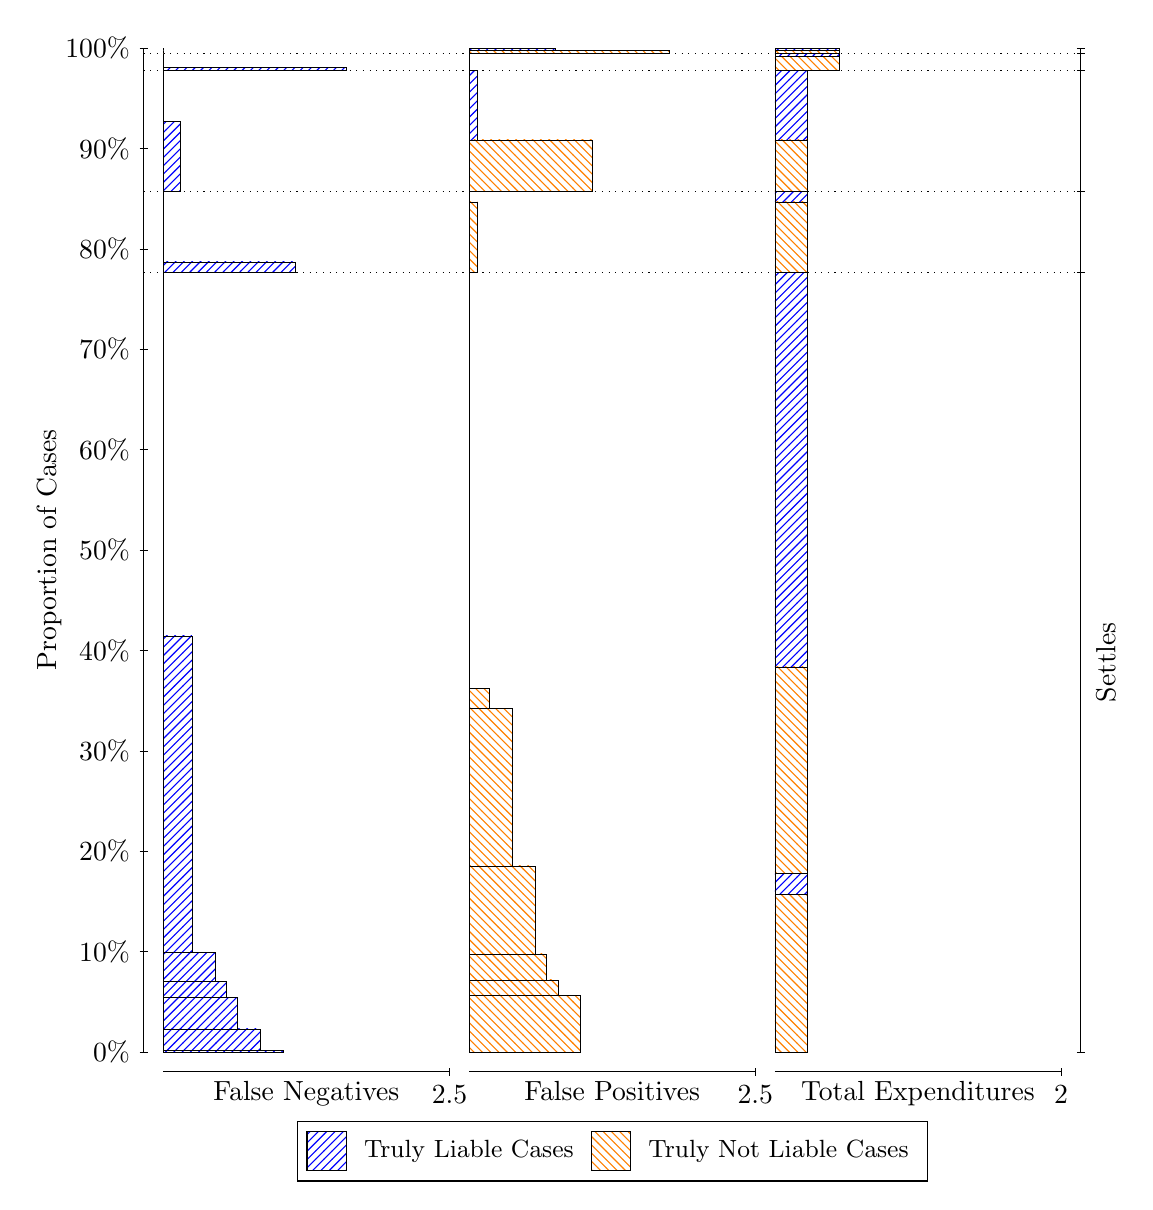
\begin{tikzpicture}
\draw[black, very thin] (1.5,1.75) -- (1.5,14.5);
\node[rotate=90, text=black, anchor=center] at (0.3, 8.125) {Proportion of Cases};
\draw[black, very thin] (1.45,1.75) -- (1.55,1.75);
\node[text=black, anchor=east] at (1.45, 1.75) {0\%};
\draw[black, very thin] (1.45,3.025) -- (1.55,3.025);
\node[text=black, anchor=east] at (1.45, 3.025) {10\%};
\draw[black, very thin] (1.45,4.3) -- (1.55,4.3);
\node[text=black, anchor=east] at (1.45, 4.3) {20\%};
\draw[black, very thin] (1.45,5.575) -- (1.55,5.575);
\node[text=black, anchor=east] at (1.45, 5.575) {30\%};
\draw[black, very thin] (1.45,6.85) -- (1.55,6.85);
\node[text=black, anchor=east] at (1.45, 6.85) {40\%};
\draw[black, very thin] (1.45,8.125) -- (1.55,8.125);
\node[text=black, anchor=east] at (1.45, 8.125) {50\%};
\draw[black, very thin] (1.45,9.4) -- (1.55,9.4);
\node[text=black, anchor=east] at (1.45, 9.4) {60\%};
\draw[black, very thin] (1.45,10.675) -- (1.55,10.675);
\node[text=black, anchor=east] at (1.45, 10.675) {70\%};
\draw[black, very thin] (1.45,11.95) -- (1.55,11.95);
\node[text=black, anchor=east] at (1.45, 11.95) {80\%};
\draw[black, very thin] (1.45,13.225) -- (1.55,13.225);
\node[text=black, anchor=east] at (1.45, 13.225) {90\%};
\draw[black, very thin] (1.45,14.5) -- (1.55,14.5);
\node[text=black, anchor=east] at (1.45, 14.5) {100\%};

\draw[black, very thin] (13.4,1.75) -- (13.4,14.5);
\draw[black, very thin] (13.35,1.75) -- (13.45,1.75);
\node[anchor=west] at (13.35, 1.75) {};
\draw[black, very thin] (13.35,11.65) -- (13.45,11.65);
\node[anchor=west] at (13.35, 11.65) {};
\draw[black, very thin] (13.35,12.68) -- (13.45,12.68);
\node[anchor=west] at (13.35, 12.68) {};
\draw[black, very thin] (13.35,14.217) -- (13.45,14.217);
\node[anchor=west] at (13.35, 14.217) {};
\draw[black, very thin] (13.35,14.428) -- (13.45,14.428);
\node[anchor=west] at (13.35, 14.428) {};
\draw[black, very thin] (13.35,14.5) -- (13.45,14.5);
\node[anchor=west] at (13.35, 14.5) {};

\draw[black, very thin, pattern color=blue, pattern=north east lines] (1.75,1.75) rectangle (3.276,1.7682);
\draw[black, very thin, pattern color=blue, pattern=north east lines] (1.75,1.7682) rectangle (2.9853,2.0431);
\draw[black, very thin, pattern color=blue, pattern=north east lines] (1.75,2.0431) rectangle (2.6947,2.4481);
\draw[black, very thin, pattern color=blue, pattern=north east lines] (1.75,2.4481) rectangle (2.5493,2.6416);
\draw[black, very thin, pattern color=blue, pattern=north east lines] (1.75,2.6416) rectangle (2.404,3.0166);
\draw[black, very thin, pattern color=blue, pattern=north east lines] (1.75,3.0166) rectangle (2.1133,7.0344);
\draw[black, very thin, pattern color=orange, pattern=north west lines] (1.75,7.0344) rectangle (1.75,11.65);
\draw[black, very thin, pattern color=blue, pattern=north east lines] (1.75,11.65) rectangle (3.4213,11.783);
\draw[black, very thin, pattern color=orange, pattern=north west lines] (1.75,11.783) rectangle (1.75,12.68);
\draw[black, very thin, pattern color=blue, pattern=north east lines] (1.75,12.68) rectangle (1.968,13.565);
\draw[black, very thin, pattern color=orange, pattern=north west lines] (1.75,13.565) rectangle (1.75,14.217);
\draw[black, very thin, pattern color=blue, pattern=north east lines] (1.75,14.217) rectangle (4.0753,14.256);
\draw[black, very thin, pattern color=orange, pattern=north west lines] (1.75,14.256) rectangle (1.75,14.428);
\draw[black, very thin, pattern color=orange, pattern=north west lines] (1.75,14.428) rectangle (1.75,14.467);
\draw[black, very thin, pattern color=blue, pattern=north east lines] (1.75,14.467) rectangle (1.75,14.5);
\draw[black, very thin, pattern color=orange, pattern=north west lines] (5.6333,1.75) rectangle (7.0503,2.4706);
\draw[black, very thin, pattern color=orange, pattern=north west lines] (5.6333,2.4706) rectangle (6.7597,2.6662);
\draw[black, very thin, pattern color=orange, pattern=north west lines] (5.6333,2.6662) rectangle (6.6143,2.9968);
\draw[black, very thin, pattern color=orange, pattern=north west lines] (5.6333,2.9968) rectangle (6.469,4.1145);
\draw[black, very thin, pattern color=orange, pattern=north west lines] (5.6333,4.1145) rectangle (6.1783,6.1114);
\draw[black, very thin, pattern color=orange, pattern=north west lines] (5.6333,6.1114) rectangle (5.8877,6.3658);
\draw[black, very thin, pattern color=blue, pattern=north east lines] (5.6333,6.3658) rectangle (5.6333,11.65);
\draw[black, very thin, pattern color=orange, pattern=north west lines] (5.6333,11.65) rectangle (5.7423,12.547);
\draw[black, very thin, pattern color=blue, pattern=north east lines] (5.6333,12.547) rectangle (5.6333,12.68);
\draw[black, very thin, pattern color=orange, pattern=north west lines] (5.6333,12.68) rectangle (7.1957,13.332);
\draw[black, very thin, pattern color=blue, pattern=north east lines] (5.6333,13.332) rectangle (5.7423,14.217);
\draw[black, very thin, pattern color=orange, pattern=north west lines] (5.6333,14.217) rectangle (5.6333,14.389);
\draw[black, very thin, pattern color=blue, pattern=north east lines] (5.6333,14.389) rectangle (5.6333,14.428);
\draw[black, very thin, pattern color=orange, pattern=north west lines] (5.6333,14.428) rectangle (8.1767,14.467);
\draw[black, very thin, pattern color=blue, pattern=north east lines] (5.6333,14.467) rectangle (6.7233,14.5);
\draw[black, very thin, pattern color=orange, pattern=north west lines] (9.5167,1.75) rectangle (9.9254,3.7469);
\draw[black, very thin, pattern color=blue, pattern=north east lines] (9.5167,3.7469) rectangle (9.9254,4.0218);
\draw[black, very thin, pattern color=orange, pattern=north west lines] (9.5167,4.0218) rectangle (9.9254,6.6407);
\draw[black, very thin, pattern color=blue, pattern=north east lines] (9.5167,6.6407) rectangle (9.9254,11.65);
\draw[black, very thin, pattern color=orange, pattern=north west lines] (9.5167,11.65) rectangle (9.9254,12.547);
\draw[black, very thin, pattern color=blue, pattern=north east lines] (9.5167,12.547) rectangle (9.9254,12.68);
\draw[black, very thin, pattern color=orange, pattern=north west lines] (9.5167,12.68) rectangle (9.9254,13.332);
\draw[black, very thin, pattern color=blue, pattern=north east lines] (9.5167,13.332) rectangle (9.9254,14.217);
\draw[black, very thin, pattern color=orange, pattern=north west lines] (9.5167,14.217) rectangle (10.334,14.389);
\draw[black, very thin, pattern color=blue, pattern=north east lines] (9.5167,14.389) rectangle (10.334,14.428);
\draw[black, very thin, pattern color=orange, pattern=north west lines] (9.5167,14.428) rectangle (10.334,14.467);
\draw[black, very thin, pattern color=blue, pattern=north east lines] (9.5167,14.467) rectangle (10.334,14.5);
\draw[black, dotted] (1.5,11.65) -- (13.4,11.65);
\draw[black, dotted] (1.5,12.68) -- (13.4,12.68);
\draw[black, dotted] (1.5,14.217) -- (13.4,14.217);
\draw[black, dotted] (1.5,14.428) -- (13.4,14.428);
\draw[black, very thin] (1.75,1.5) -- (5.3833,1.5);
\node[text=black, anchor=north] at (3.5667, 1.5) {False Negatives};
\draw[black, very thin] (5.3833,1.45) -- (5.3833,1.55);
\node[text=black, anchor=north] at (5.3833, 1.45) {2.5};

\draw[black, very thin] (5.6333,1.5) -- (9.2667,1.5);
\node[text=black, anchor=north] at (7.45, 1.5) {False Positives};
\draw[black, very thin] (9.2667,1.45) -- (9.2667,1.55);
\node[text=black, anchor=north] at (9.2667, 1.45) {2.5};

\draw[black, very thin] (9.5167,1.5) -- (13.15,1.5);
\node[text=black, anchor=north] at (11.333, 1.5) {Total Expenditures};
\draw[black, very thin] (13.15,1.45) -- (13.15,1.55);
\node[text=black, anchor=north] at (13.15, 1.45) {2};

\node[text=black, centered, rotate=90] at (13.72, 6.7001) {Settles};





\draw (7.449999999999999,1.5) node[draw=none] (baseCoordinate) {};
\begin{scope}[align=center]
        \matrix[scale=0.5, draw=black, below=0.5cm of baseCoordinate, nodes={draw}, column sep=0.1cm]{
            \node[rectangle, draw, minimum width=0.5cm, minimum height=0.5cm, pattern color=blue, pattern=north east lines] {}; &
            \node[draw=none, font=\small, text=black] (B) {Truly Liable Cases}; &
            \node[rectangle, draw, minimum width=0.5cm, minimum height=0.5cm, pattern color=orange, pattern=north west lines] {}; &
            \node[draw=none, font=\small, text=black] (B) {Truly Not Liable Cases}; \\
            };
\end{scope}

\end{tikzpicture}
\end{document}